%% ----------------------------------------------------------------
%% Thesis.tex -- MAIN FILE (the one that you compile with LaTeX)
%% ---------------------------------------------------------------- 

% Set up the document
\documentclass[a4paper, 11pt, oneside]{Thesis}  % Use the "Thesis" style, based on the ECS Thesis style by Steve Gunn
\graphicspath{Figures/}  % Location of the graphics files (set up for graphics to be in PDF format)

% Include any extra LaTeX packages required
\usepackage[square, numbers, comma, sort&compress]{natbib}  % Use the "Natbib" style for the references in the Bibliography
\usepackage{verbatim}  % Needed for the "comment" environment to make LaTeX comments
\usepackage{vector}  % Allows "\bvec{}" and "\buvec{}" for "blackboard" style bold vectors in maths
\hypersetup{urlcolor=blue, colorlinks=true}  % Colours hyperlinks in blue, but this can be distracting if there are many links.
\usepackage{url}
\usepackage{hyperref}
\newcommand\fnurl[2]{
	\footnote{\href{#2}{#1}}
}

%% ----------------------------------------------------------------
\begin{document}
\frontmatter      % Begin Roman style (i, ii, iii, iv...) page numbering

% Set up the Title Page
\title  {Fordypningsprosjekt}
\authors  {\texorpdfstring
            {\href{esbena@stud.ntnu.no}{Esben Aarseth}}
            {Esben Aarseth}
            {aleksg@stud.ntnu.no}{Aleksander Gisvold}
            {Aleksander Gisvold}
            }
\addresses  {\groupname\\\deptname\\\univname}  % Do not change this here, instead these must be set in the "Thesis.cls" file, please look through it instead
\date       {\today}
\subject    {}
\keywords   {}

\maketitle
%% ----------------------------------------------------------------

\setstretch{1.3}  % It is better to have smaller font and larger line spacing than the other way round

% Define the page headers using the FancyHdr package and set up for one-sided printing
\fancyhead{}  % Clears all page headers and footers
\rhead{\thepage}  % Sets the right side header to show the page number
\lhead{}  % Clears the left side page header

\pagestyle{fancy}  % Finally, use the "fancy" page style to implement the FancyHdr headers

%% ----------------------------------------------------------------
% Declaration Page required for the Thesis, your institution may give you a different text to place here
\Declaration{

\addtocontents{toc}{\vspace{1em}}  % Add a gap in the Contents, for aesthetics

I, AUTHOR NAME, declare that this thesis titled, `THESIS TITLE' and the work presented in it are my own. I confirm that:

\begin{itemize} 
\item[\tiny{$\blacksquare$}] This work was done wholly or mainly while in candidature for a research degree at this University.
 
\item[\tiny{$\blacksquare$}] Where any part of this thesis has previously been submitted for a degree or any other qualification at this University or any other institution, this has been clearly stated.
 
\item[\tiny{$\blacksquare$}] Where I have consulted the published work of others, this is always clearly attributed.
 
\item[\tiny{$\blacksquare$}] Where I have quoted from the work of others, the source is always given. With the exception of such quotations, this thesis is entirely my own work.
 
\item[\tiny{$\blacksquare$}] I have acknowledged all main sources of help.
 
\item[\tiny{$\blacksquare$}] Where the thesis is based on work done by myself jointly with others, I have made clear exactly what was done by others and what I have contributed myself.
\\
\end{itemize}
 
 
Signed:\\
\rule[1em]{25em}{0.5pt}  % This prints a line for the signature
 
Date:\\
\rule[1em]{25em}{0.5pt}  % This prints a line to write the date
}
\clearpage  % Declaration ended, now start a new page

%% ----------------------------------------------------------------
% The "Funny Quote Page"
\pagestyle{empty}  % No headers or footers for the following pages

\null\vfill
% Now comes the "Funny Quote", written in italics
\textit{``Gotta Catch `Em All''}

\begin{flushright}
- Ash Ketchum
\end{flushright}

\vfill\vfill\vfill\vfill\vfill\vfill\null
\clearpage  % Funny Quote page ended, start a new page
%% ----------------------------------------------------------------

% The Abstract Page
\addtotoc{Abstract}  % Add the "Abstract" page entry to the Contents
\abstract{
\addtocontents{toc}{\vspace{1em}}  % Add a gap in the Contents, for aesthetics

The Thesis Abstract\ldots
\paragraph{Keywords:}
\emph{BLOPP, Asthma}

}

\clearpage  % Abstract ended, start a new page
%% ----------------------------------------------------------------

\setstretch{1.3}  % Reset the line-spacing to 1.3 for body text (if it has changed)

% The Acknowledgements page, for thanking everyone
\acknowledgements{
\addtocontents{toc}{\vspace{1em}}  % Add a gap in the Contents, for aesthetics

We would like to thank \ldots

}
\clearpage  % End of the Acknowledgements
%% ----------------------------------------------------------------

\pagestyle{fancy}  %The page style headers have been "empty" all this time, now use the "fancy" headers as defined before to bring them back


%% ----------------------------------------------------------------
\lhead{\emph{Contents}}  % Set the left side page header to "Contents"
\tableofcontents  % Write out the Table of Contents

%% ----------------------------------------------------------------
\lhead{\emph{List of Figures}}  % Set the left side page header to "List if Figures"
\listoffigures  % Write out the List of Figures

%% ----------------------------------------------------------------
\lhead{\emph{List of Tables}}  % Set the left side page header to "List of Tables"
\listoftables  % Write out the List of Tables

%% ----------------------------------------------------------------
\setstretch{1.5}  % Set the line spacing to 1.5, this makes the following tables easier to read
\clearpage  % Start a new page
\lhead{\emph{Abbreviations}}  % Set the left side page header to "Abbreviations"
\listofsymbols{ll}  % Include a list of Abbreviations (a table of two columns)
{
% \textbf{Acronym} & \textbf{W}hat (it) \textbf{S}tands \textbf{F}or \\
\textbf{NTNU} & \textbf{N}orwegian \textbf{U}niversity of \textbf{S}cience and \textbf{T}echnology \\
\textbf{BLOPP} & \textbf{B}arns \textbf{L}egemiddel\textbf{OPP}levelser
\textbf{CAPP} & \textbf{C}hild \textbf{APP}lication
\textbf{GAPP} & \textbf{G}uardian \textbf{APP}lication

}

%% ----------------------------------------------------------------
% End of the pre-able, contents and lists of things
% Begin the Dedication page

\setstretch{1.3}  % Return the line spacing back to 1.3

\pagestyle{empty}  % Page style needs to be empty for this page
\dedicatory{To Pikachu!}

\addtocontents{toc}{\vspace{2em}}  % Add a gap in the Contents, for aesthetics


%% ----------------------------------------------------------------
\mainmatter	  % Begin normal, numeric (1,2,3...) page numbering
\pagestyle{fancy}  % Return the page headers back to the "fancy" style

% Include the chapters of the thesis, as separate files
% Just uncomment the lines as you write the chapters

\chapter{Introduction}
\label{chp:introduction}

This chapter will give an introduction to the study. It will state the purpose, motivation, research questions and the research method for this study. 

\section{Purpose}
\label{sec:purpose}
The goal of this study is to evaluate the CAPP, GAPP and Karotz Applications created by Aaberg, Aarseth, Dale, Gisvold and Svalestuen \cite{CustomerDriven}.
The evaluation will be done through usability testing carried out on all three applications. The results of these initial tests will thereafter be used to improve the applications for a newer version. 
We will also plan a thorough testing of the applications.


\section{Motivation}
\label{sec:motivation}
According to NAAF, 20\% \cite{NAAF} of the Norwegian population has or has had asthma at the age of 10, and 8\% of the adult population suffers from asthma. Many of the children find it unpleasant to use their medicine as they often do not understand why the medicine must be taken [Should have a reference]. This may result in parents applying the medication incorrectly, applying the wrong treatment, or even forgetting to give the medicine to their children. 


\section{Research Questions}
\label{sec:researchquestions}
The main goal for this study is to evaluate the CAPP, GAPP and Karotz application, and identify the usability problems in these systems. Structuring the goal into different research questions will help this study with the evaluation of the goal. The goal has been composed into these questions:

\paragraph{RQ1:}
\textbf{How will guardians of a child react on having a Karotz constantly ``watching'' over their child?}


\paragraph{RQ2:}
\textbf{What will I have for lunch today?}

This evaluation should be done through user testing and feedback from future users of the applications. The testing will give information on how well the 
\ldots

\section{Research Method}
\label{sec:researchmethod}


 % Introduction

\chapter{Background}
\label{chp:background}


This chapter will give a brief introduction to the history behind the BLOPP project [insert reference] and the CAPP, GAPP and Karotz applications.


\section{BLOPP Project}
\label{sec:bloppproject}
Barns Legemiddelopplevelser is a project group ...

\subsection{CAPP/GAPP/Karotz project}
In the fall of 2012 Aaberg, Aarseth, Dale, Gisvold and Svalestuen were engaged by the BLOPP Project group through the course TDT4290 - Customer Driven Project \cite{customerdrivenntnu} at NTNU. In the period of august 2012 to December 2012 they developed a tangible medical reminder named CAPP/GAPP/KAPP. A full report of their work is available at [Insert Reference]. 
Their prototype is the foundation for our work in this project.


\section{CAPP/GAPP/KAPP}
\label{sec:cappgappkapp}
The prototype mentioned in the previous section resulted in three separate applications named CAPP, GAPP and KAPP. These are described in an overview below.  

\subsection{GAPP}
GAPP is an Android application targeted towards the parents or guardians of the children. 
Its basic functionality is to view logs of how often a child needs medication, how the child has been feeling the latest couple of days, according to the asthma traffic light system, and to set up alarms for the child. 
CAPP and GAPP works together as a pair, so a child may only have one parent and vice versa. %Er siste setning nødvendig?


\subsection{CAPP}
CAPP is an Android application targeted towards the children. It launches the alarms given by parents and guides children during their medication. After a medication is complete, the child gets a star in its treasure chest.    

%PICTURES, OR IT DIDN'T HAPPEN!


\subsection{KAPP}
KAPP is another application targeted towards children. The application runs on a Karotz\cite{karotz}, which is a small robot bunny \ref{fig:karotz}. The purpose of the Karotz is to give reminders to children when it is time to take their asthma medicine and give instructions during treatment. In order to interact with the Karotz, children may use either a Nanoz (a small bunny with an integrated RFID) or by pressing a button on the top of the Karotz' head.    



\subsection{Known areas for improvement}
\label{sec:improvements}
As Aaberg, Aarseth, Dale, Gisvold and Svalestuen finished their work, they commented on several areas of potential improvement for CAPP/GAPP/KAPP. This document is reprinted in its entirety in Appendix \ref{app:furtherWork} (after permission from Aaberg, Aarseth, Dale, Gisvold and Svalestuen). The main topics for improvement were
\begin{enumerate}
\item{Reward System}
\item{Distraction sequence for children}
\item{Web application}
\item{Support for more children}
\end{enumerate}

These comments are used as a basis when we decide what to improve in this project. 
%In addition, we have discovered a potential in sending out emails with records, which perhaps will go directly to the child's doctor. Hvor skal vi skrive om dette? 


\section{Existing products}
\label{sec:exisiting-products}

On the two biggest application stores, Google Play and iOS AppStore, we have found a couple of applications similar to the one we have in mind. Among the ones we have looked into, is Huff and Puff \fnurl{Google Play : Huff And Puff}{https://play.google.com/store/apps/details?id=com.healthnutsmedia.huffandpuffsd.free}, Asthma Logger
\fnurl{Google Play : Asthma Logger}{https://play.google.com/store/apps/details?id=org.androworks.asthmalog}, Kids Beating Asthma \fnurl{Google Play : Kids Beating Asthma}{https://play.google.com/store/apps/details?id=es.medianet.hcsc01} and Asthma Monitor \fnurl{Google Play : Asthma Monitor}{https://play.google.com/store/apps/details?id=ch.imvs.unibas.asthma}. Common for all these applications is that they have one specific aim. For instance, Huff and Puff wants to teach children in general about asthma. Asthma Logger logs treatments, and Kids Beating Asthma have some game elements, but the games are not available for playing during treatment. For our product, we want to create a superset of these applications. 

\begin{sidewaystable}
	\label{tab:existing-product-table}
	\begin{tabular}{ | p{4.0cm} | p{5.5cm} | p{5.5cm} | p{4cm}|}
	\hline
	\textbf{Application} & \textbf{Positive} & \textbf{Negative} & \textbf{Target Audience} \\ \hline
	
   Huff And Puff 
	& 
	\begin{itemize}
	  \item Relevant quizzes from introduction to more experienced users
	  \item Can play sounds if children cannot read
	  \item Has asthma-specific word games, puzzles, etc.  
	\end{itemize}
	&
	\begin{itemize}
	  \item Poor navigation models
	  \item Quiz is too generic, for instance asks what doctors call this and that.
	  \item The games are not exactly what we look for, as they cannot be played while undergoing a treatment  
	\end{itemize}
	&
	Children
	\\ \hline
	Asthma Logger
	& 
	\begin{itemize}
	  \item Possibility to send journal on email specified by user. May forward the journal to doctor.  
	  \item Very intuitive application
	  \item Shows doses taken the last couple of days
	\end{itemize}
	& 
	\begin{itemize}
	  \item Only has one generic medicine (does not state which medicine, for instance Ventoline) or dosage (?) 
	\end{itemize}
	& 
	Adults
	\\ \hline
	Kids Beating Asthma
	& 
	\begin{itemize}
	  \item Informative and simple
	\end{itemize}
	&
	\begin{itemize}
	  \item Suffers from software bugs and crashes regularly
	\end{itemize}
	& Children
	\\ \hline
	Asthma Monitor
	&
	\begin{itemize}
	  \item Ability connect Peak Flow to activities
	  \item Thorough and ``advanced'' statistics
	  \item Can input symptoms like Cough, Sputum, Wheezing breath and Dyspnsea 
	  \item Can send records via email
	\end{itemize}
	&
	\begin{itemize}
	  \item Old fashioned GUI
	\end{itemize}
	& 
	Adults
	\\ \hline
	\end{tabular}
	\caption{Evaluation of existing products on the market}
\end{sidewaystable}

\subsection{Conclusion and evaluation}
\label{sec:existingconcl}

The main ideas we want to take further in our application are the email-sending system of Asthma Logger and the quiz-aspect of Huff And Puff. In general, it is a good idea to be able to send your journal on email, for instance to yourself. If we combine this with possibility to send the journal to a doctor, we have a great time saving tool. To give an example: Ole has been feeling ill for a while, and has been logging when he takes his medicine. He can then schedule an appointment with his doctor, and send his journal on email to the doctor. When he arrives to his appointment, the doctor already knows how many times he has taken his medicine the last days and can give advice based upon these facts. 

Asthma Monitor seems like a great application once you get used to it, and it is developed by researchers, which implies that they know what they're doing. However, it seems a bit too complex for the following reasons:
\begin{enumerate}
  \item If an adult who have no other experience of asthma other than through his/her child, the application contains terminology which they might not be very used to
  \item The user interface is not very appealing
  \item Forcing information from a child regarding how much they cough once a day seems rather hard 
\end{enumerate}   

As for the quiz, we have concluded that this is a great way to inform children. Namely by letting them playing around with the application and gathering knowledge on this basis. 

\subsection{Assessment of existing applications}
In 2012, Huckvale et. al. \cite{huckvale2012apps} conducted an assesment on the existing applications on both Google Play and AppStore. They assessed 103 different apps with english as the native language. Out of these 103, \emph{No apps for people with asthma combined reliable, comprehensive information about the condition with supportive tools for self­management.}(Huckvale et. al., 2012). They concluded that doctors should be careful when recommending apps for people with the purpose of self management. 






 % Background Theory 

\chapter{Usability}
\label{chp:usability}

This chapter will give a brief definition of what usability is, and how user tests can help us improve it. Since are applications are targeted towards both children and adults, we will give a description of how the usability tests for these groups will differ. We will also explain how the user testing is performed at \ldots

\section{What is usability?}
There are many ways to describe usability. 

The International Organization for Standardization(ISO) has a definition of the term usability \cite{isousability}:

Extent to which a system, product or service can be used by specified
users to achieve specified goals with effectiveness, efficiency
and satisfaction in a specified context of use.

The same document defines the context of use as:

Users, tasks, equipment (hardware, software and materials), and
the physical and social environments in which a product is used.

These definitions cover how the system is used, the user's thoughts about the use and the context of the system. This can be broken further down into several subgoals in order to achieve better usability, and to give us a better insight on what usability is. 
These subgoals are:

\begin{enumerate}
\item{How precise is the user able to perform a task using the application?}
\item{How much resources(for example time, or number of tries) was used to perform the given task using the application?}
\item{How many errors occurred?}
\item{Did the user find the use satisfactory?}
\end{enumerate}

User-centered design is a way of designing with the user in mind. By using this technique these goals are achievable. User-centered design is about getting feedback from the users during the design and development process. Always thinking about how the user would solve this problem, and consolidate the users when in doubt is a fundamental part of user-centered design. The user's opinion is the measure of how good the system performs and the user's feedback defines how you score on usability. [Should have reference]

\section{How to test usability}
There are many ways to create a good user experience. Having knowledge of expert opinions is always a good idea, and using user-centered design techniques are also a wise way to go. According to SOME PERSON [Insert Reference] developers should get feedback from users by users tests at different stages of development. According to SOME PERSON [Insert reference], having a user-centered approach will help the developers to address the weakest parts of their system, and give feedback on design decisions. 

A user-centered design can be done in many different ways, at different stages of the product life cycle \cite{abrasusercentereddesign}, as shown in Table \ref{table:designduringlifecycle}:

\begin{table}[H]
\begin{tabular}{|p{5cm} | p{5cm} | p{5cm} |}
\hline
\textbf{Method} & \textbf{Purpose} & \textbf{Phase of the project lifecycle} \\ \hline
Background interviews and questionnaires & To collect data and to understand the user better & When starting the project \\ \hline
Focus groups & Discover design issues and receive feedback & At an early stage \\ \hline
On-site observation & To both collect information of the context the system will be used in, and find the primary problems the users have & At an early stage \\ \hline
Role playing / simulations & Will give a broader understanding of what the user expects from the system & Early to mid stage of the project \\ \hline
Automated evaluation & Gives feedback on deviations from standards or best practices. This method exclude actual users, but are based on well tested principles & Mid to end of the project \\ \hline
Usability testing & To measure the usability of your system and provide feedback on very specific elements that are badly designed & Abras \cite{abrasusercentereddesign} says it should be at the end of the project while others \cite{schneidermanusercentered} thinks it should be done in iterations throughout the project. \\ \hline
Interviews and questionnaires & Gives a qualitative measurement of how good or bad the system is & End of the project \\ \hline
\end{tabular}
\caption{Methods of user-centered feedback}
\label{table:designduringlifecycle}
\end{table}

The purpose of this project is to test an existing system, improve the existing product and plan an extensive testing of the improved product. We will focus mainly on WHAT WHAT WHAT?

\paragraph{Usability Testing}
The purpose of usability testing is to increase the usability of a system. At the same time, performing these usability tests can save the developers some time and reduce the cost of the project by removing errors and poor design at an early stage \cite{dumas1995practical}.

The usability testing can be performed in different ways \cite{schneidermanusercentered}. At early stages of the project, low-fidelity prototypes are a good option since they will provide feedback and take proportionally little time to make, making it easier to have more iterations of testing. The different testing methods include a potential user of the system performing tasks to provide real data. Observing and recording each usability test can help the developers to analyze their system, and correct the flaws \cite{dumas1995practical}. 

Before starting the usability tests, the developers should set goals planning what they want to know about the system \cite{isosoftwareengineering}. This will ensure that the purpose of the test is fulfilled. The developers should then plan tasks according to the desired results. These tasks should allow the user to explore the system, or the parts the developers want to test, giving the test person some time per task, in order to not stress the test person. 

After being planned, the test should be run on a number of different test persons. From figure %\ref{figure:numberoftests}
, you can see that as the number of participants increases, the number of undetected errors decrease. 

%%
%\begin{figure}[H]
%\begin{center}
%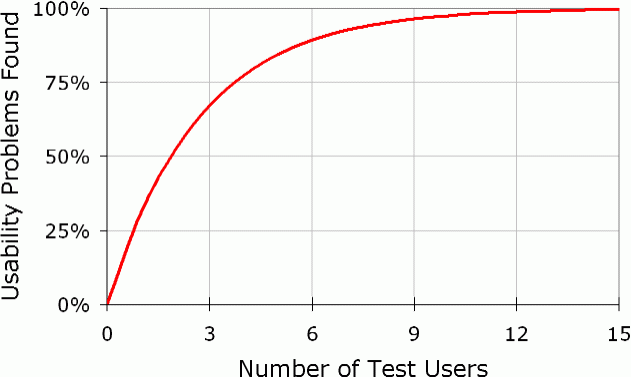
\includegraphics{Thesis/Pictures/numberoftests}
%\end{center}
%\caption{Number of users needed to find percentage of errors[Insert reference]}
%\label{numberoftests}
%\end{figure}

Nielsen states that after five user tests, 85\% of the errors have been found \cite{nielsennumberoftests}. Molich\cite{molich2008usable} states that six test persons is the ultimate number. 

\paragraph{Testing environment}
\label{par:testingenvironment}
The next thing to consider when performing usability testing is the testing environment. It should resemble the environment in which the system will be used. To make the most of the tests, it is wise to perform videotaping of the tests. This will help when reviewing the results from the test[insert references]. If the test are being recorded, a consent from the test person will be necessary.

Before the test persons arrive, a test leader should be chosen, in order to have a person to guide the test persons through the process. The test leader should be in charge of testing and act as an interviewer to help the participant ``think-aloud''\footnote{Reference to Thinking aloud}. The test leader should answer questions from the participant, but be careful not to give away information that will affect the results of the test.

After the tasks are done, it is necessary to gather loose ends and get answers to all the questions that might be unanswered. A system usability scale(SUS)\cite{sus} can be a good way to grade the usability of the system together with the observations made during the test. The SUS scale will reflect on how satisfying the usability is in the eyes of the users. Bangor et al \cite{susform} have made a scale based on the SUS-forms from different system usability tests, in order to make it possible to compare the mean score of a system with what is an acceptable level of usability. In our testing, we will make use of a Norwegian version, developed by Svanæs \ref{chp:norsksus}.

\section{How to test usability on children and toddlers}
While usability testing on children and toddlers have the same basic approach as testing on adults, there are many more precautions to be followed. 
Hanna et al. \cite{testingenvironmentforchildren} lays out some of these precautions. They recommend not using children that are skilled with computers since they may find the tasks to easy and will not give useful data. 
Since children these days have a higher skill with computers thanks to the invasion of tablets and smart phones [insert reference?], this may not as much of a concern. 

Since our application is targeted towards children suffering from Asthma, we want to test the system on children suffering from Asthma, in addition to, children from the same age group, not suffering from Asthma. These children will most certainly have a different approach to the system and may give different feedback.

Hanna, Risden and Alexander also point out changed that should be made to the testing environment as mentioned in \ref{par:testingenvironment}. They recommend making the testing environment more child friendly by placing colourful posters on the walls.
Children of young age may be afraid of ``The Doctor's Office'' and we will need to make adjustments to avoid children being scared upon arrival at the test lab. 

As mentioned by Donker and Markopoulos \cite{TalkAloud} talk-aloud is very useful technique when doing usability testing with children. Talk-aloud is a technique were the children talk about what they are doing instead of what they are thinking.

THIS NEEDS MORE WORK

\section{NSEP Usability Lab}
\label{nseplab}

This section will describe some of the features in the NSEP Usability Lab, used by NTNU to perform usability testing. 

\subsection{The Facility}
I made this section Justin Case. % Usability

%\input{Chapters/Chapter4} % Experiment 1

%\input{Chapters/Chapter5} % Experiment 2

\chapter{Results and Discussion}
\label{resultsanddiscussion}

This chapter will go through the findings from this study and summarize the results to answer the research questions from Section \ref{reseachquestions}


\section{Evaluation}


\section{Research Method}


 % Results and Discussion

\chapter{Conclusions}
\label{conclusions} % Conclusion

%% ----------------------------------------------------------------
% Now begin the Appendices, including them as separate files

\addtocontents{toc}{\vspace{2em}} % Add a gap in the Contents, for aesthetics

\appendix % Cue to tell LaTeX that the following 'chapters' are Appendices

\chapter{An Appendix}	% Appendix Title

\chapter{Further Work}
\label{app:furtherWork}
This chapter gives an overview of some of the ideas both the customer and the developers had for further development of the application. This includes a description of further development, analysis of the user groups and work towards NAAF and the health department.
The main part of the work to be done after the end of this project is connected to requirements that has been taken out of this project due to limitation of time and resources. Other issues remaining is connected to the security and privacy of the patient's treatment log and storing sensitive information.
Section \ref{sec:frcompleted} lists the overall requirements that have not been implemented during the project. These requirements has either been requested early in the process of have been brought up during discussions and meetings with the stakeholders. 


% Here goes the major potential improvements such as privacy/security, rewardsystem and connection
\section{Improvements}
\label{sec:Improvements}
The following sections describes the ideas we had for future improvements to the applications. It is parted into subsections for improvements in the fields of database records, the reward system, the distraction and the web application.

%\input{FurtherWork/WebAccess}
%\input{FurtherWork/SecurityAndPrivacy}

\subsection{Rewardsystem}
The children's application (CAPP) is all about changing the children's view of medication to something positive. It shall be a motivation for the children to take their medication. It is therefore an important task to entertain them and give them some form of reward when they take their medication. As for now, we have given stars to the child after completed medication. The stars are in a treasure chest where the child can see how many stars he or she has. This is a simple reward, but worked fairly well during the user tests. However, it may be boring over time. 

The initial idea was to have a shop where the children could buy clothes and other items to their avatar. The stars earned from finishing treatments would serve as credits in the shop. This was not implemented due to time restrictions. It is also possible to take this to the real world, e.g. that the child gets a lollipop for every 10th star, but this would have to be supervised by the parents. 
 

There is an endless line of opportunities for this reward system, and we chose the simplest implementation, so we would have something to test. 

\subsection{Distraction sequence for children}
During our workshop, we came up with a lot of ideas for distractions for the children. These would range from simple animation sequences, like what we decided to implement, to more complex 
things like games that would not require a lot of movement and could therefore help during longer treatments. 

The distraction sequence is one of the fields were we feel it has more or less never ending possibilities for improvement, and as more research into what children finds distracting, but not to the point 
where they can't take their medicine, this distraction sequence can be evolved.


\subsection{User testing of the guardian application}
GAPP has not yet been user tested on actual parents of asthmatic children. This has to be done to get an understanding of how they interact with the system, and to get knowledge about what they think of an application of this type. This is a system to make it easier for the guardians to give their children medications. While it is important that the children likes the system, it is also important that the parents feel it helps them give their children their medicines, without it being a big time waster.

\subsection{Web application}
There is a possibility of making this application as a web application, as a whole. By extracting the functionality and running it on a web service it would make it easier for people to use it across platforms. Done right, it may run on all devices with an internet connection. This may also give an easier integration with external information such as air pollution forecast, pollen forecast, temperatures, etc. Since our application is written in Java, using Android SDK, it will not run on an internet server as is. Making a web application will require an almost complete refactoring of the source code.

 
\subsection{Support for more children}
Currently, the application only use one child, but there are implemented support for using more children. Each child has its own id (childId), and support for more children can be implemented without much change of the existing code. There should also be concidered using accounts for the guardians connected to the children, in case of the guardians having more than one asthmatic child. 
  

% Here goes the minor ideas and improvements for further work
\section{Ideas and minor improvements}


\begin{description}

\item[Webinterface] The doctors may prefer to set up the users medication plans through a web interface on their computers. This part may be integrated into existing systems. 

\item[Other devices] The application are fitted for a phone running the Android operating system. For the future it should also be scalable to tablets. There may be more interesting for a child to work on a tablet than a phone. There will also be much more space for content. This extra space gives greater potential of the reward system. It should also be available on other operating systems than Android, e.g. iOS or Windows Phone. This will improve the availability for the users, not limiting them to Android phones. 

\item[Overall graphical design] The priorities have been to make the major functionality work. We have used lots of time making the applications understandable and easy to use, but there is still a great potential in making the applications interaction design better. 

\item[Personalize the system] The application may be more personalized. E.g. "It's time to take medication" could be "It's time to take medication, Eric". By involving the users name more in the system, they may feel more appreciated. 

\item[Integration of external elements] The distraction part of the application may be integrated with a story or other external elements. I. eg. a story where the children will need to take medicine in order to get the next part of the story.

\end{description}


 % Further Work on CAPP/GAPP/KAPP

%\input{Appendices/AppendixC} % Appendix Title

\addtocontents{toc}{\vspace{2em}}  % Add a gap in the Contents, for aesthetics
\backmatter

%% ----------------------------------------------------------------
\label{Bibliography}
\lhead{\emph{Bibliography}}  % Change the left side page header to "Bibliography"
\bibliographystyle{unsrtnat}  % Use the "unsrtnat" BibTeX style for formatting the Bibliography
\bibliography{Bibliography}  % The references (bibliography) information are stored in the file named "Bibliography.bib"

\end{document}  % The End
%% ----------------------------------------------------------------